% !TEX root = ../main.tex

% Indicate the main file. Must go at the beginning of the file.

%--------------------------------------------------------------------------------
% CHAPTER Results
%--------------------------------------------------------------------------------


\chapter{Prototyp Sniffer} % Protoypen Test Main chapter title -> Sniffer Prototyp!?
\label{Prototyp Sniffer} % Change X to a consecutive number; for referencing this chapter elsewhere, use \ref{ChapterX}

%---------------------------------------------------------------------------------
% SECTION 1
%---------------------------------------------------------------------------------

\section{ESP32}
\label{sec:ResultatESP32}
%\textcolor{red}{Erstes Resultat des ESP: SPI ist nicht genügend schnell, um die Packete des FPGA entgegen zu nehmen}

Der Test der Firmware des ESP32-S3 wurde gemäss Kapitel \ref{sub:ESPSPIundFSMTest} durchgeführt. Als Erstes wurde das kurze Telegramm getestet und der Pin 21 wurde nicht auf Ground verbunden. Durch Drücken der Boot-Taste wird das Senden getriggert. In Abbildung \ref{fig:ResultatBLEKurz} ist die Anzeige in der Applikation \textit{Bluetility} gezeigt und Einfärbungen gemacht, welche Teile zu den Daten gehören.

\begin{figure}[H]
    \centering
    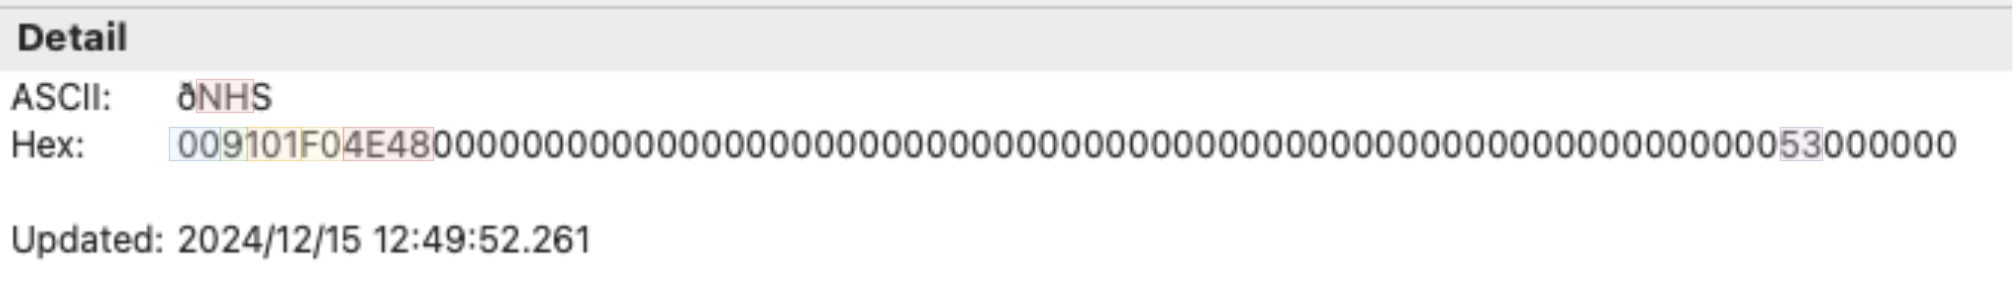
\includegraphics[width=0.9\linewidth]{Figures/Chap4/ESP32/Resultat_BLE_kurz.png}
    \caption{Resultat Bluetility kurzes Telegram}
    \label{fig:ResultatBLEKurz}
\end{figure}

Die Aufzeichnung der Reaktionszeit für das kurze Telegramm mit dem Osziloskop ist in Abbildung \ref{ffig:ReakKurz} zu sehen. Die gelbe Linie ist dabei die \textit{Chip Select} Leitung und die blaue Linie die \textit{Handshakeleitung}. 

\begin{figure}[H]
    \centering
    % Erstes Bild
    \begin{subfigure}[b]{0.45\textwidth}
        \centering
        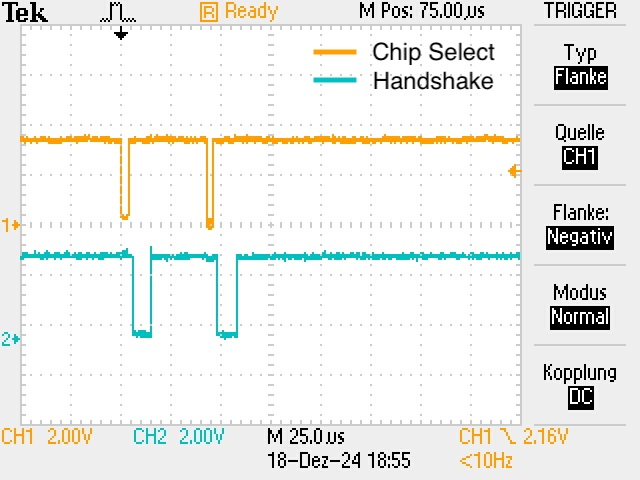
\includegraphics[width=\linewidth]{Figures/Chap4/ESP32/Gesammte Transaktion Kurz.JPG} 
        \caption{Insgesamt 2 Transaktionen}
        \label{fig:GesTransKurz}
    \end{subfigure}
    \hfill 
    %Zweites Bild
    \begin{subfigure}[b]{0.45\textwidth}
        \centering
        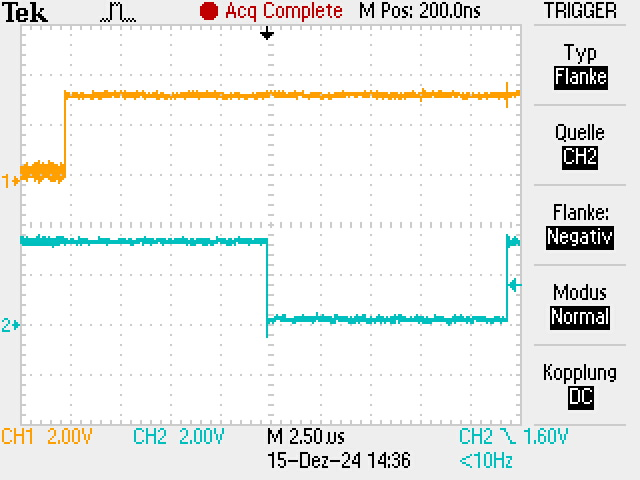
\includegraphics[width=\linewidth]{Figures/Chap4/ESP32/Reaktionszeit Kurz.JPG} 
        \caption{Vergrösserung im Zeitbereich der Reaktionszeit bei kurzem Telegramm}
        \label{fig:ReakKurz}
    \end{subfigure}
    \caption{Resultat der Reaktionszeit kurzes Telegramm gemessen mit dem Osziloskop}
    \label{fig:ResultatOsziReaktionKurz} 
\end{figure}

In Abbildung \ref{fig:GesTransKurz} ist ersichtlich, dass das vollständige Telegramm nach 2 Transaktionen abgeschlossen ist. In Abbildung \ref{fig:ReakKurz} beträgt die Reaktionszeit zwischen Transaktionsende, wenn die Chip Select Leitung eine positive Flanke hat, und der Verarbeitung der Daten, wenn die Handshakeleitung eine negative Flanke hat, 10 $\mu$s. Die Zeit zwischen der positiven Flanke der CS Leitung und der positiven Flanke der Handshake Leitung beträgt ungefähr 24 $\mu$s.


Als Zweites wurde das Lange Telegramm getestet. In Abbildung \ref{fig:ResultatBLELang} ist die Anzeige in der Applikation \textit{Bluetility} gezeigt und Einfärbungen gemacht, welche Teile zu den Daten gehören.

\begin{figure}[H]
    \centering
    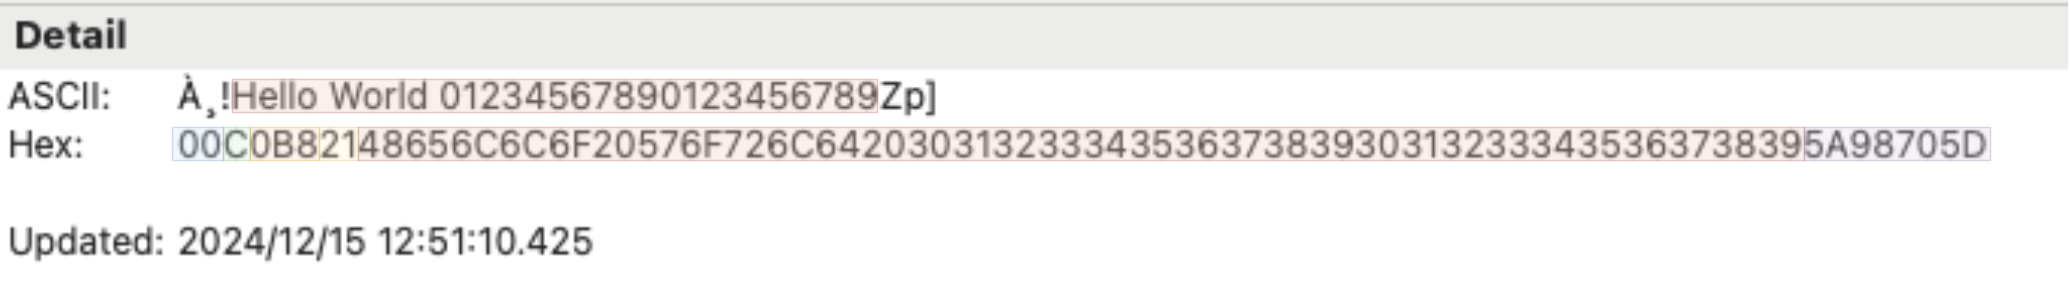
\includegraphics[width=0.9\linewidth]{Figures/Chap4/ESP32/Resultat_BLE_lang.png}
    \caption{Resultat Bluetility langes Telegram}
    \label{fig:ResultatBLELang}
\end{figure}

Die Aufzeichnung der Reaktionszeit für das kurze Telegramm mit dem Osziloskop ist in Abbildung \ref{fig:ReakLang} zu sehen. Die gelbe Linie ist dabei die \textit{Chip Select} Leitung und die blaube Linie die Handshakeleitung 

\begin{figure}[H]
    \centering
    % Erstes Bild
    \begin{subfigure}[b]{0.45\textwidth}
        \centering
        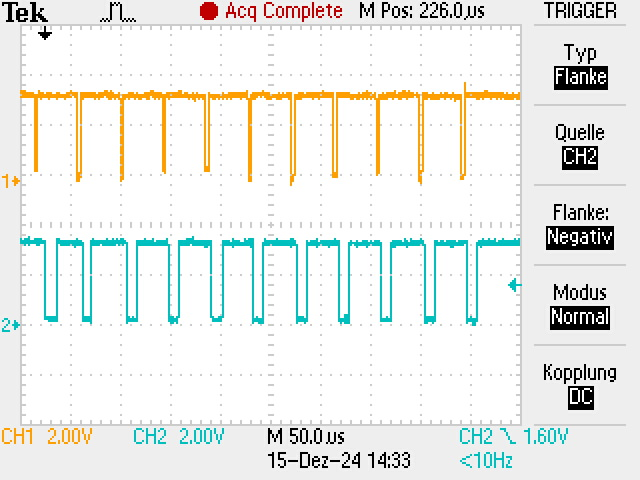
\includegraphics[width=\linewidth]{Figures/Chap4/ESP32/Gesammte Transaktion Lang.JPG} 
        \caption{Insgesamt 11 Transaktionen}
        \label{fig:GesTransLang}
    \end{subfigure}
    \hfill 
    %Zweites Bild
    \begin{subfigure}[b]{0.45\textwidth}
        \centering
        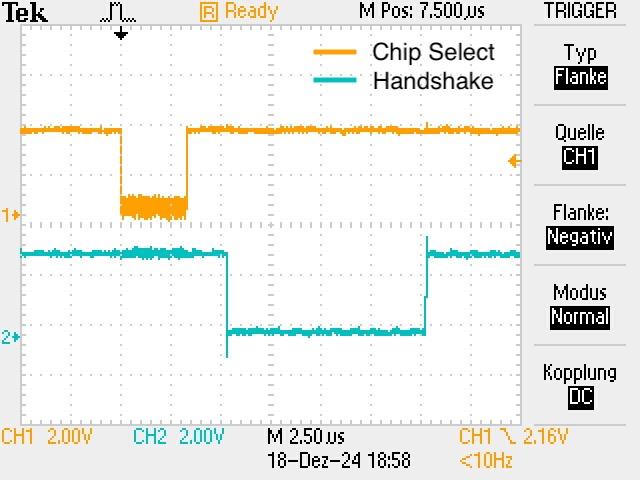
\includegraphics[width=\linewidth]{Figures/Chap4/ESP32/Reaktionszeit Lang.JPG} 
        \caption{Vergrösserung im Zeitbereich der Reaktionszeit bei langem Telegramm}
        \label{fig:ReakLang}
    \end{subfigure}
    \caption{Resultat der Reaktionszeit langem Telegramm gemessen mit dem Osziloskop}
    \label{fig:ResultatOsziReaktionLang} 
\end{figure}

In Abbildung \ref{fig:GesTransLang} sind 11 Transaktionen zu sehen, für die 11 Negativen pulse der Chip Select Leitung. Dies ist die Anzahl Transitionen, die benötigt werden, um ein langes Telegramm zu übermitteln. Die Reaktionszeit in Abbildung \ref{fig:ReakLang} sind gleich wie beim kurzen Telegramm: 10 $\mu$s und ungefähr 24 $\mu$s.


%\href{https://docs.espressif.com/projects/esp-idf/en/stable/esp32s3/api-reference/peripherals/spi_slave.html#transaction-interval}{ESP-IDF SPI Slave Transaction Interval}



%---------------------------------------------------------------------------------
% SECTION 2
%---------------------------------------------------------------------------------
\section{FPGA}
\label{sec:ResultatFPGA}



\section{Hardware Sniffer}
\label{sec:ResultatHardware}




\section{Übertragungstest SPI}
\label{sec:ResultatÜbertragungSPI}







% \section{Resultat} % 
% \textcolor{red}{Was ist beim Test herausgekommen. Was hat funktionniert, was nicht?}

